\documentclass[12pt]{article}

% Packages
% ---
\usepackage{amsmath} % Advanced math typesetting
\usepackage[utf8]{inputenc} % Unicode support (Umlauts etc.)
\usepackage[french]{babel} % Change hyphenation rules
\usepackage{hyperref} % Add a link to your document
\usepackage{graphicx} % Add pictures to your document
\usepackage{listings} % Source code formatting and highlighting
\usepackage{fancybox}
\usepackage{subfig}
\usepackage[margin=1in]{geometry}
\usepackage{wrapfig}

%\DeclareGraphicsExtensions{.png}
\captionsetup[figure]{textfont=it}

\title{Rapport du travail pratique 1 : Série de Fourier}
\date{\today}
\author{Présenté par Philippe Caron\\dans le cadre du cours Traitement du signal (IFT3205)\\Université de Montréal}

\begin{document}
\begin{titlepage}
  \maketitle
  \thispagestyle{empty}
\end{titlepage}

\section{Visualisation \& Propriété de la Transformée de Fourier}
\setcounter{subsection}{1}
\subsection{Fonction de recentrage}
Il y a deux méthodes évidentes pour remettre les quatres coins de l'image au centre. On peut soit déplacer les quadrants selon un « X » tel que suggéré dans la donnée du TP, ou alors les renverser en effectuant une symétrie autour de la droite qui relie les deux coins du quadrant qui correspondent au milieu du côté de l'image:

\begin{figure}[ht]
  \centering
  \shadowbox{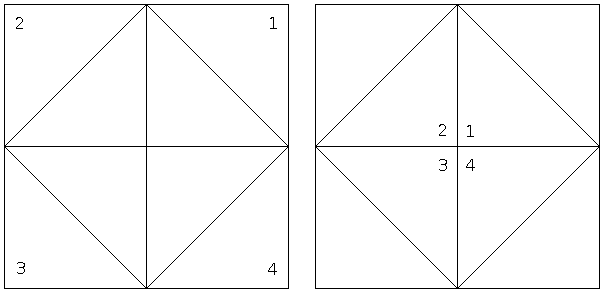
\includegraphics[height = 2cm]{methode2.png}}
  \captionsetup{width=.8\linewidth}
  \caption[width = 8cm]{Dans ce cas-ci les quadrants ne changent pas de position, mais sont pivotés sur eux-même autour de la ligne noire qui les divise}
\end{figure}

Étant donné que le résultat de la transformée de Fourier est symétrique, il n'y a aucun avantage à choisir la seconde méthode. Qui plus est, la première est plus facile et plus simple à implémenter, en plus d'être plus rapide. Le choix est donc facile à faire et c'est la méthode suggérée dans le TP qui a été implémentéeé. En voici le résultat sur la première image:

\begin{figure}[ht]
  \centering
  \subfloat[Avant]{\shadowbox{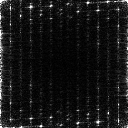
\includegraphics[height = 3cm]{pascentree.png}}}
  \hspace{.5cm}
  \subfloat[Après]{\shadowbox{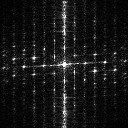
\includegraphics[height = 3cm]{centree.png}}}
  \captionsetup{width=.8\linewidth}
  \caption{Comparaison du module de D1r.pgm avant et après l'application de CenterImg}
\end{figure}

Comme on peut le constater, la fonction de recentrage est efficace. L'appel de CenterImg à nouveau permet de retrouver la Figure 2(a).
\pagebreak

\subsection{Fonction logarithmique}
Pour pouvoir utiliser la fonction Log sans avoir à réutiliser Recal, elle a été définie comme suit:
\begin{equation}
  I(x, y) = f \cdot \ln{(I(x, y))}
\end{equation}
où $f = 255 \div \ln{255}$ afin que tous les pixels soient élevés à la valeurs qu'ils occuperaient sur 255. Voici le résultat de l'application de cette fonction sur le module de D1r.pgm:

\begin{figure}[ht]
  \centering
  \shadowbox{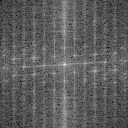
\includegraphics[height = 3cm]{loga.png}}
  \captionsetup{width=.8\linewidth}
  \caption{On voit bien plus clairement les ligne verticales vers les extrémités de la photo comparée à la version avant l'application du log (Figure 2(b))}
\end{figure}

La clareté des bandes verticales semble indiquer une forte répétition du motif horizontal. Le fait que la ligne du centre soit particulièrement claire indique une quantité élevée de basse fréquences, ce qui peut-être expliqué par le fait que la couleur générale de l'image n'est pas régulière. Cependant, on remarque que les lignes verticales sont perpendiculaires au motif horizontal et que leur espacement rappel celui du motif horizontal.

\pagebreak

\subsection{Correspondance}
Voici les images avant et après le calcul du module auxquelles la fonction Log a été appliquée.
\begin{figure}[ht]
  \centering
  \subfloat[]{\shadowbox{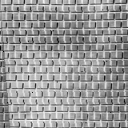
\includegraphics[height = 3cm]{a.png}}}
  \hspace{0.5cm}
  \subfloat[]{\shadowbox{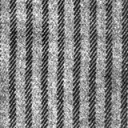
\includegraphics[height = 3cm]{b.png}}}
  \hspace{0.5cm}
  \subfloat[]{\shadowbox{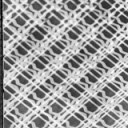
\includegraphics[height = 3cm]{c.png}}}
  \captionsetup{width=.8\linewidth}
  \caption{Les trois images D1r.pgm, D11r.pgm et D46r.pgm avant avoir été modifiées}
\end{figure}
\begin{figure}[ht]
  \centering
  \subfloat[]{\shadowbox{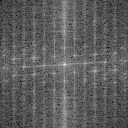
\includegraphics[height = 3cm]{loga.png}}}
  \hspace{0.5cm}
  \subfloat[]{\shadowbox{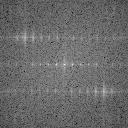
\includegraphics[height = 3cm]{logb.png}}}
  \hspace{0.5cm}
  \subfloat[]{\shadowbox{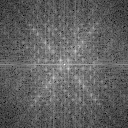
\includegraphics[height = 3cm]{logc.png}}}
  \captionsetup{width=.8\linewidth}
  \caption{Les trois images D1r.pgm, D11r.pgm et D46r.pgm après avoir été modifiées}
\end{figure}

\subsubsection{(a)}
\begin{wrapfigure}[9]{l}{8em}
  \centering
  \shadowbox{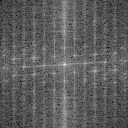
\includegraphics[height = 3cm]{loga.png}}
  \caption{}
\end{wrapfigure}
Tel que discuté plus haut, on voit que cette image semble avoir une forte redondance sur l'axe vertical. On voit aussi une ligne un peu oblique près de l'horizontale, ce qui suggère également un motif de l'image originale dans cet angle (on voit l'espace entre les briques de l'image (a) se décaler avec le même angle). Les fréquences reviennent selon un motif très régulier, donc il y a une dominance claire d'une fréquence puis de ses harmoniques, et puisque celles-ci continuent très loin vers les extrémité, on peut supposer que cette l'image originale est composée d'un motif très régulier.

\vspace{2cm}

\subsubsection{(b)}
\begin{wrapfigure}[10]{l}{8em}
  \centering
  \shadowbox{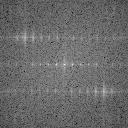
\includegraphics[height = 3cm]{logb.png}}
  \caption{}
\end{wrapfigure}
Cette image est sans doute la plus abstraite des trois. Il semble y avoir très peu d'information par rapport aux deux autres, donc probablement une image plus simple. On voit quand même des ligne horizontales assez définie, donc un motif vertical assez clair. Elle sont assez éloignée du centre ce qui indique une haute fréquence, ces ligne sont fonc probablement causée par les petits traits dans les grosses lignes. On voit aussi qu'à l'intérieur des ligne horizontale, il y a une multitude de lignes verticales, donc il y a également un motif horizontal, celui-ci est évident. Si on regarde attentivement on voit un losange au centre, et deux points plus brillant dans l'axe perpendiculaire aux côtés du losange. Si on interprète ceci comme étant une troisième ligne on peut déduire la présence d'un motif dans le sens du côté du losange le plus défini. C'est probablment du au fait que l'on peut poursuivre chaque trait composant les lignes principales pour aboutir sur un autre de sorte qu'il y a un motif pointillé.

\subsubsection{(c)}
\begin{wrapfigure}[7]{l}{8em}
  \centering
  \shadowbox{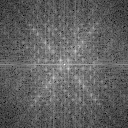
\includegraphics[height = 3cm]{logc.png}}
  \caption{}
\end{wrapfigure}
S'il fallait associer chaque image à son spectre sans les images d'origine, celle-ci serait probablement la plus facile à trouver. Il est évident qu'il y a un motif à peu prêt à 45 degrés, ce qui distingue immédiatement cette image des deux autres. On remarque aussi une ligne relativement claire à l'horizontale, mais il ne semble pas y avoir de différence notable entre l'horizontale et la verticale dans l'image originale, cette ligne est probablement due à la barre noire à gauche de l'image originale.

\vspace{2cm}

\subsubsection {En résumé}
Il semble y avoir une corrélation importante entre les lignes visible dans le spectre et le motif dans l'image originale. Ce doit être parce que la présence d'un motif augmente beaucoup la quantité de fréquences utiles à sa génération le long de son « chemin » ce qui explique pourquoi les lignes sont toujours perpendiculaires au motif. De plus, les images dont les spectres sont parsemés de petits points régulièrement espacés ont des propriétés de quadrillé. Il semblerait donc que les points indiquent la répétition de quadrillage. D'ailleurs cela semble « réciproque »; on dirait que les lignes dans le spectre représentent des répétitions de points, alors que les points du spectre représentent des répétitions de ligne.

\pagebreak

\section{Manipulation d'harmoniques}
Afin de manipuler efficacement les harmoniques, il est utile de concevoir quelques filtres. Au cours de la prochaine section, tous les filtres seront appliqués à l'image suivante:
\vspace{1.5cm}

\begin{figure}[ht]
  \centering
  \shadowbox{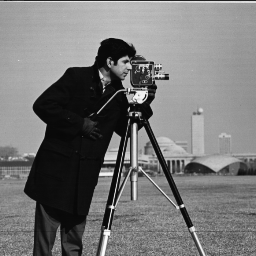
\includegraphics[height = 5cm]{photograph.png}}
  \captionsetup{width=.8\linewidth}
  \caption{Image originale de la photographie du photographe}
\end{figure}

\vspace{.5cm}

\subsection{Application des filtres}

\subsubsection{Filtre carré}
Afin de répondre à ce numéro, le filtre carré SquareFilter a été créé. Il permet de filtrer l'intérieur ou l'extérieur d'un carré dont la taille est définie en paramètre, centré dans l'image. Lorsqu'appliqué il donne le résultat suivant:
\begin{figure}[ht]
  \centering
  \shadowbox{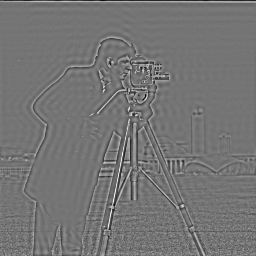
\includegraphics[height = 4cm]{2a.png}}
  \captionsetup{width=.8\linewidth}
  \caption{Résultat de l'image filtrée en supprimant les basses fréquences avec le filtre carré}
\end{figure}
La supression des basses fréquences fait disparaître la « couleur » le l'image, mais semble rehausser les countours. L'application du filtre ajoute également un effet d'onde à l'image.

\subsubsection{Filtre rond}
Pour cette image, le filtre rond sera utilisé, et à l'inverse du numéro précédent, ce seront les hautes fréquences qui seront supprimées. Voici le résultat:
\begin{figure}[ht]
  \centering
  \shadowbox{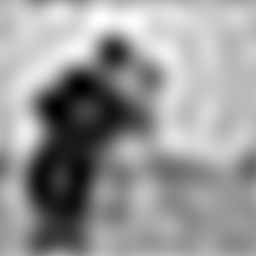
\includegraphics[height = 4cm]{2b.png}}
  \captionsetup{width=.8\linewidth}
  \caption{Résultat de l'image filtrée en supprimant les hautes fréquences avec le filtre rond}
\end{figure}
La supression des haute fréquences produit un résultat sans surprise très flou. Le filtre rond produit le même effet d'onde que le filtre carré.

\subsubsection{Filtre cône}
Le filtre appliqué ici change de valeur en fonction de la distance avec le centre, ce qui lui donnerait l'aspect d'un cône s'il était représenté en trois dimensions. Il accentue exponentiellement la valeur des hautes fréquences en les multipliant par elles-mêmes. Il produit le résultat suivant:
\begin{figure}[ht]
  \centering
  \shadowbox{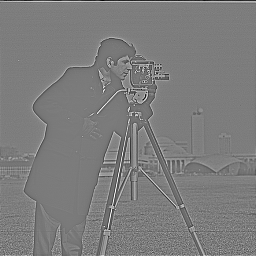
\includegraphics[height = 4cm]{2c.png}}
  \captionsetup{width=.8\linewidth}
  \caption{Résultat de l'image filtrée en accentuant les hautes fréquences avec le filtre cône}
\end{figure}
Comme pour le filtre carré plus haut, en donnant plus d'importance aux hautes fréquences les contours sont accentués, cependant les nuances de gris sont perdues, donnant l'impression d'une image monotone. Il est intéressant de noter toutefois que l'effet d'onde mentionné dans les deux questions précédente est parti. Il y a donc probablement un lien entre la coupure net d'un filtre et l'apparition de cet effet. 

\subsubsection{Filtre horizontal}
Dans les deux derniers numéros, on utilise un filtre barre qui élimine les fréquences qui sont à l'extérieur de 10px autour de l'un des axes, horizontal dans le cas présent.
\begin{figure}[ht]
  \centering
  \shadowbox{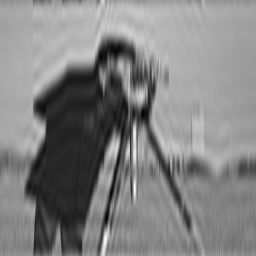
\includegraphics[height = 4cm]{2d.png}}
  \captionsetup{width=.8\linewidth}
  \caption{Résultat de l'image filtrée en supprimant les fréquences prêt de l'axe horizontal}
\end{figure}
Les effets de ce filtre auraient pu être prédit à partir des numéros précédents: la perte de hautes fréquences à engendre un flou. Par contre, le flou est seulement vertical étant donné que les fréquences qui étaient sur l'axe vertical sont toujours intacte. L'effet de vague est aussi présent ce qui renforce l'hypothèse qui veut que ce soit la coupure nette qui engendre cet effet.

\subsubsection{Filtre vertical}
On s'attend à voir la même chose mais avec un flou horizontal:
\begin{figure}[ht]
  \centering
  \shadowbox{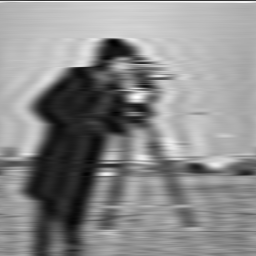
\includegraphics[height = 4cm]{2e.png}}
  \captionsetup{width=.8\linewidth}
  \caption{Résultat de l'image filtrée en supprimant les fréquences prêt de l'axe vertical}
\end{figure}

\pagebreak
\subsection{Isolation d'une fréquence}
L'image représente une fonction sinusoïdale allant dans une direction autour de 1:2, la façon la plus simple de repoduire cette image est d'isoler la fréquence qui correspond à cette fonction. Puis il suffit de procéder à tâtons en gardant toujours en tête le ratio. La fonction utilisée pour générer l'image est la suivante:
\begin{equation}
  F(x, y) = \left\{
  \begin{array}{ll}
    1$ si $x = 0.005 \cdot L$, $y = 0.01 \cdot H\\
    0$ sinon$
  \end{array}
  \right.
\end{equation}
où $L$ et $H$ sont la hauteur et la largeur respectivement. Voici le résultat obtenu:
\begin{figure}[ht]
  \centering
  \shadowbox{
\includegraphics[height = 3cm]{2.png}}
  \captionsetup{width=.8\linewidth}
  \caption{Résultat de l'image dont une seule fréquence a été isolée}
\end{figure}

\pagebreak
\section{Fréquences Spatiales}
\subsection{Monrstein}
Cette image ressemble de loin à Marilyn Monroe et de prêt à Albert Einstein. Ces deux personnages sont pourtant très différents. En fait, on ne voit de Marilyn Monroe que la silouhette, et d'Albert Einstein que les traits. C'est pourquoi en plissant les yeux ou en regardant de loin on croit voir celle-là et qu'en regardant de prêt on voit celui-ci. En terme de fréquences spatiales, Monroe est définie par les basses fréquences, ce qui lui donne la « couleur » tandis qu'Einstein lui est défini par les hautes fréquences, qui donnent le countour. Heureusement, dans le numéros précédent, un filtre a été trouvé qui correspond à chacun des effets recherchés

\subsection{Marilyn Monroe}
Pour ne conserver que les basses fréquences, nous utiliserons le filtre rond, comme utilisé plus haut, avec un rayon de 20. Afin d'enlever l'effet d'onde, le filtre cone a été testé mais le résultat (quoique sans vagues) semblait trop flou par rapport au filtre rond ordinaire. Voici le résultat:
\vspace{3cm}
\begin{figure}[ht]
  \centering
  \shadowbox{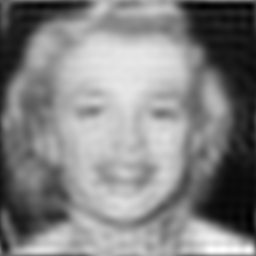
\includegraphics[height = 6cm]{Marilyn.png}}
  \captionsetup{width=.8\linewidth}
  \caption{Marilyn est extraite de l'image}
\end{figure}

\pagebreak
\subsection{Albert Einstein}
Ici, on sait que le filtre cône va fonctionner, mais au lieu d'appliquer une fonction directement proportionnelle à la distance, on applique une fonction carrée (ce qui transforme en quelque sorte le filtre cône en filtre sphère), afin de vraiment donner de l'importance aux plus hautes fréquences, mais tout en empêchant l'effet d'onde. Le résultat donné par ce filtre est très correct, mais comme dans le numéro 2, l'image produite est très monotone, c'est pourquoi l'image a été normalisée avec la fonction suivante:
\begin{equation}
  I(x, y) = (I(x, y) - 127)^f
\end{equation}
pour donner le résultat que voici:
\vspace{3cm}
\begin{figure}[ht]
  \centering
  \subfloat[Avant normalisation]{\shadowbox{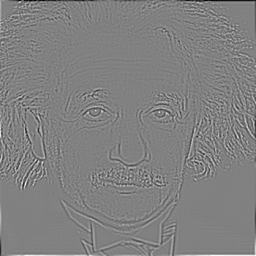
\includegraphics[height = 5cm]{Albertavant.png}}}
  \hspace{1cm}
  \subfloat[Après normalisation]{\shadowbox{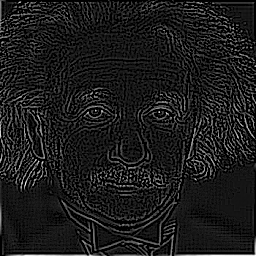
\includegraphics[height = 5cm]{Albert.png}}}
  \captionsetup{width=.8\linewidth}
  \caption{Albert est séparé de la photo}
\end{figure}

\end{document}

